\documentclass{standalone}

\usepackage{tikz}
\usetikzlibrary{positioning}
\usetikzlibrary{er}

%% Grid spacing
\newdimen\ERspacing
\ERspacing=3cm

\begin{document}
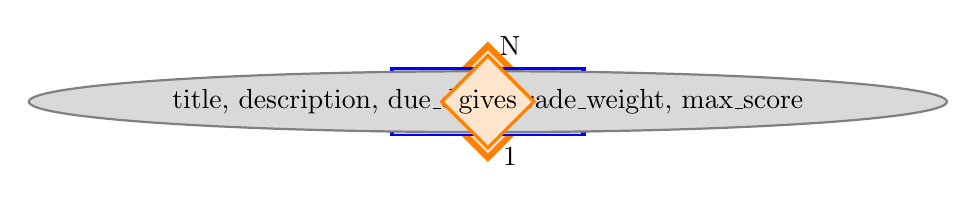
\begin{tikzpicture}
    [
    node distance=\ERspacing and \ERspacing,
    on grid,
    every entity/.style={fill=blue!20, draw=blue, thick},
    every relationship/.style={fill=orange!20, draw=orange, very thick},
    every attribute/.style={fill=gray!30, draw=gray, thick},
    ]

    \node[entity] (ent_user)
    {User}
    child {node [attribute, left = 2\ERspacing of ent_user] {name, email, password}};
    
    \node[relationship, below = of ent_user] (rel_has_role)
    {role}
    edge (ent_user)
    child {node [entity, below = of rel_has_role] (ent_student) {Student}}
    child {node [entity, below right = of rel_has_role] (ent_admin) {Admin}}
    child {node [entity, below left = of rel_has_role] (ent_professor) {Professor}};

    \node [xshift=0.8em, yshift=-2em] at (ent_user) {1};
    \node [xshift=0.8em, yshift=2em] at (rel_has_role) {N};

    \node[relationship, below = of ent_professor] (rel_teaches)
    {teaches}
    edge (ent_professor);

    \node[entity, below = of rel_teaches] (ent_class)
    {Class}
    edge (rel_teaches)
    child {node[attribute, right = 2\ERspacing of ent_class] {dates, status, max\_students}};

    \node[relationship, below = of ent_student] (rel_enrolls)
    {enrolls}
    edge (ent_student)
    edge (ent_class)
    child {node [attribute, right = 2\ERspacing of rel_enrolls] {date, status, grade, priority}};

    \node[relationship, below = of ent_class] (rel_courses)
    {courses}
    edge (ent_class)
    child {node [entity, right = of rel_courses] (ent_course) {Course}};

    \node[attribute, below right = of ent_course] {course\_code, title, description, max\_students}
    edge (ent_course);

    \node[relationship, left = of ent_class] (rel_has)
    {has}
    edge (ent_class);

    \node[entity, left = of rel_has] (ent_material)
    {Class Material}
    edge (rel_has)
    child {node [attribute, above = of ent_material] {title, description, file\_url}};

    \node[entity, below left = of rel_has] (ent_activity)
    {Class Activity}
    edge (rel_has)
    child {node [attribute, below = of ent_activity] {title, description, due\_date, grade\_weight, max\_score}};

    \node[left = 4\ERspacing of ent_professor, inner sep = 0pt, outer sep = 0pt] (anchor1) {} edge (ent_professor);
    \node[relationship, below = 2\ERspacing of anchor1] (rel_gives)
    {gives}
    edge (anchor1)
    edge (ent_material)
    edge (ent_activity);
\end{tikzpicture}
\end{document}
